\tikzstyle{input_neuron}=[circle,draw=red!50,fill=orange!10,thick,minimum size=.2mm]
\tikzstyle{hidden_neuron}=[circle,draw=blue!50,fill=blue!10,thick,minimum size=1mm]
\tikzstyle{output_neuron}=[circle,draw=green!50,fill=green!20,thick,minimum size=1mm]			
\tikzstyle{input}=[circle,draw=black!50,fill=black!20,thick,minimum size=.2mm]
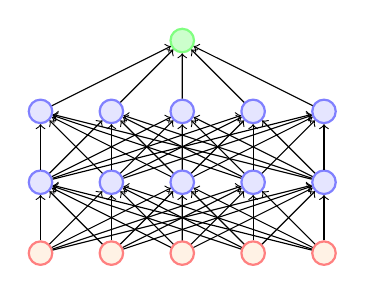
\begin{tikzpicture}[scale=.9, transform shape]
	%\tikzstyle{every node} = [draw,shape=circle]
	\node[input_neuron] (a0) at (0, 0) {};
	\node[input_neuron] (a1) at (1, 0) {};
	\node[input_neuron] (a2) at (2, 0) {};
	\node[input_neuron] (a3) at (3, 0) {};
	\node[input_neuron] (a4) at (4, 0) {};
	\node[hidden_neuron] (b0) at (0, 1) {};
	\node[hidden_neuron] (b1) at (1, 1) {};
	\node[hidden_neuron] (b2) at (2, 1) {};
	\node[hidden_neuron] (b3) at (3, 1) {};
	\node[hidden_neuron] (b4) at (4, 1) {};
	\node[hidden_neuron] (c0) at (0, 2) {};
	\node[hidden_neuron] (c1) at (1, 2) {};
	\node[hidden_neuron] (c2) at (2, 2) {};
	\node[hidden_neuron] (c3) at (3, 2) {};
	\node[hidden_neuron] (c4) at (4, 2) {};
	\node[output_neuron] (d2) at (2, 3) {};
	\foreach \from in {a0,a1,a2,a3,a4}
	\foreach \to in {b0,b1,b2,b3,b4}
	\draw [->] (\from) -- (\to);
	\foreach \from in {b0,b1,b2,b3,b4}
	\foreach \to in {c0,c1,c2,c3,c4}
	\draw [->] (\from) -- (\to);
	\foreach \from in {c0,c1,c2,c3,c4}
	\draw [->] (\from) -- (d2);
\end{tikzpicture}